\def\slidemode{
  \documentclass[fleqn,aspectratio=169]{beamer}
\usepackage{pgfpages}
}
\def\handoutmode{
  \documentclass[handout,fleqn,aspectratio=169]{beamer}
\usepackage{pgfpages}
\pgfpagesuselayout{resize to}[a4paper,landscape,border shrink=5mm]
}


%\def\pdfmode{handoutmode}
\def\pdfmode{slidemode}

\csname\pdfmode\endcsname

\mode<presentation>
{
  \usetheme{default}
  \usecolortheme{default}
  \usefonttheme{default}
  \setbeamertemplate{navigation symbols}{}
  \setbeamertemplate{caption}[numbered]
  \setbeamertemplate{footline}[frame number]  % or "page number"
  \setbeamercolor{frametitle}{fg=white}
  \setbeamercolor{footline}{fg=black}
} 


\usepackage[english]{babel}
%\usepackage[utf8x]{inputenc}
\usepackage{tikz}
\usepackage{courier}
\usepackage{array}
\usepackage{bold-extra}
%\usepackage{minted}
%\usepackage[thicklines]{cancel}
%\usepackage{fancyvrb}
\usepackage{kotex}
\usepackage{paralist}
\usepackage{collectbox}
\usepackage{amsmath}
\usepackage{mathtools}
\usepackage{nccmath}
\usepackage{bm}
\usepackage{booktabs}
\usepackage{tcolorbox}
\usepackage[absolute,overlay]{textpos}

\xdefinecolor{dianablue}{rgb}{0.18,0.24,0.31}
\xdefinecolor{darkblue}{rgb}{0.1,0.1,0.7}
\xdefinecolor{darkgreen}{rgb}{0,0.5,0}
\xdefinecolor{darkgrey}{rgb}{0.35,0.35,0.35}
\xdefinecolor{darkorange}{rgb}{0.8,0.5,0}
\xdefinecolor{darkred}{rgb}{0.7,0,0}
\definecolor{darkgreen}{rgb}{0,0.6,0}
\definecolor{mauve}{rgb}{0.58,0,0.82}


\title[]{Lecture 0: Introduction}
\author{Yi, Yung (이융)}
\institute{EE210: Probability and Introductory Random Processes\\ KAIST EE}
\date{\today}

%%%%%%%%%%%% real, integer notation
\newcommand{\real}{{\mathbb R}}
\newcommand{\integer}{{\mathbb Z}}

%%% set, vector, matrix
\newcommand{\set}[1]{\ensuremath{\mathcal #1}}
\renewcommand{\vec}[1]{\bm{#1}}
\newcommand{\mat}[1]{\bm{#1}}


%%% big parenthesis
\def\Bl{\Bigl}
\def\Br{\Bigr}
\def\lf{\left}
\def\ri{\right}


%%% floor notations
\newcommand{\lfl}{{\lfloor}}
\newcommand{\rfl}{{\rfloor}}
\newcommand{\floor}[1]{{\lfloor #1 \rfloor}}

%%% gradient
\newcommand{\grad}[1]{\nabla #1}

%%% definition
\newcommand{\eqdef}{\ensuremath{\triangleq}}
%%% imply
\newcommand{\imp}{\Longrightarrow}



\newcommand{\separator}{
%  \begin{center}
    \par\noindent\rule{\columnwidth}{0.3mm}
%  \end{center}
}

\newcommand{\mynote}[1]{{\it \color{red} [#1]}}







%%% equation alignment
\newcommand{\aleq}[1]{\begin{align*}#1\end{align*}}

%%%%%%%%%%%%%%%% colored emphasized font, blanked words

\newcommand{\empr}[1]{{\color{red}\emph{#1}}}
\newcommand{\empb}[1]{{\color{blue}\emph{#1}}}

%normal colored text
\newcommand{\redf}[1]{{\color{red} #1}}
\newcommand{\yellowf}[1]{{\color{yellow} #1}}
\newcommand{\bluef}[1]{{\color{blue} #1}}
\newcommand{\grayf}[1]{{\color{gray} #1}}
\newcommand{\magenf}[1]{{\color{magenta} #1}}
\newcommand{\greenf}[1]{{\color{green} #1}}
\newcommand{\cyanf}[1]{{\color{cyan} #1}}
\newcommand{\orangef}[1]{{\color{orange} #1}}


\newcommand{\blk}[1]{\underline{\mbox{\hspace{#1}}}}


\newcommand{\redblk}[1]{\framebox{\color{red} #1}}
\newcommand{\redblank}[2]{\framebox{\onslide<#1->{\color{red} #2}}}
\newcommand{\blueblk}[1]{\framebox{\color{blue} #1}}
\newcommand{\blueblank}[2]{\framebox{\onslide<#1->{\color{blue} #2}}}



\makeatletter
\newcommand{\mybox}{%
    \collectbox{%
        \setlength{\fboxsep}{1pt}%
        \fbox{\BOXCONTENT}%
    }%
}
\makeatother

\makeatletter
\newcommand{\lecturemark}{%
    \collectbox{%
        \setlength{\fboxsep}{1pt}%
        \fcolorbox{red}{yellow}{\BOXCONTENT}%
    }%
}
\makeatother

\usepackage{tcolorbox}
\newcommand{\mycolorbox}[1]{
\begin{tcolorbox}[colback=red!5!white,colframe=red!75!black]
#1
\end{tcolorbox}
}

%%%% figure inclusion
\newcommand{\mypic}[2]{
\begin{center}
\includegraphics[width=#1\textwidth]{#2}
\end{center}
}

\newcommand{\myinlinepic}[2]{
\makebox[0cm][r]{\raisebox{-4ex}{\includegraphics[height=#1]{#2}}}
}


%%%% itemized and enumerated list
\newcommand{\bci}{\begin{compactitem}}
\newcommand{\eci}{\end{compactitem}}
\newcommand{\bce}{\begin{compactenum}}
\newcommand{\ece}{\end{compactenum}}


%%%% making 0.5/0.5 two columns
%%%% how to use: first number: length of separation bar
% \mytwocols{0.6}
% {
% contents in the left column
% }
% {
% contents in the right column
% }
%%%%
\newcommand{\mytwocols}[3]{
\begin{columns}[T] \column{.499\textwidth} #2 \column{.001\textwidth} \rule{.3mm}{{#1}\textheight} \column{.499\textwidth} #3 \end{columns}}

\newcommand{\mythreecols}[4]{
\begin{columns}[T] \column{.31\textwidth} #2 \column{.001\textwidth} \rule{.3mm}{{#1}\textheight} \column{.31\textwidth} #3 \column{.001\textwidth} \rule{.3mm}{{#1}\textheight} \column{.31\textwidth} #4  \end{columns}}

\newcommand{\mysmalltwocols}[3]{
\begin{columns}[T] \column{.4\textwidth} #2 \column{.001\textwidth} \rule{.3mm}{{#1}\textheight} \column{.4\textwidth} #3 \end{columns}}

%%%% making two columns with customized ratios
%%%% how to use:
%first parameter: length of separation bar
%second parameter: ratio of left column
%third parameter: ratio of right column
% \mytwocols{0.6}{0.7}{0.29}
% {
% contents in the left column
% }
% {
% contents in the right column
% }
%%%%
\newcommand{\myvartwocols}[5]{
\begin{columns}[T] \column{#2\textwidth} {#4} \column{.01\textwidth} \rule{.3mm}{{#1}\textheight} \column{#3\textwidth} {#5} \end{columns}}

%%% making my block in beamer
%%% first parameter: title of block
%%% second parameter: contents of block
\newcommand{\myblock}[2]{
\begin{block}{#1} {#2}  \end{block}}

%%% independence notation
\newcommand{\indep}{\perp \!\!\! \perp}

%%%% probability with different shapes (parenthesis or bracket) and different sizes
%%% `i' enables us to insert the subscript to the probability
\newcommand{\bprob}[1]{\mathbb{P}\Bl[ #1 \Br]}
\newcommand{\prob}[1]{\mathbb{P}[ #1 ]}
\newcommand{\cbprob}[1]{\mathbb{P}\Bl( #1 \Br)}
\newcommand{\cprob}[1]{\mathbb{P}( #1 )}
\newcommand{\probi}[2]{\mathbb{P}_{#1}[ #2 ]}
\newcommand{\bprobi}[2]{\mathbb{P}_{#1}\Bl[ #2 \Br]}
\newcommand{\cprobi}[2]{\mathbb{P}_{#1}( #2 )}
\newcommand{\cbprobi}[2]{\mathbb{P}_{#1}\Bl( #2 \Br)}

%%%% expectation with different shapes (parenthesis or bracket) and different sizes
%%% `i' enables us to insert the subscript to the expectation
\newcommand{\expect}[1]{\mathbb{E}[ #1 ]}
\newcommand{\cexpect}[1]{\mathbb{E}( #1 )}
\newcommand{\bexpect}[1]{\mathbb{E}\Bl[ #1 \Br]}
\newcommand{\cbexpect}[1]{\mathbb{E}\Bl( #1 \Br)}
\newcommand{\bbexpect}[1]{\mathbb{E}\lf[ #1 \ri]}
\newcommand{\expecti}[2]{\mathbb{E}_{#1}[ #2 ]}
\newcommand{\bexpecti}[2]{\mathbb{E}_{#1}\Bl[ #2 \Br]}
\newcommand{\bbexpecti}[2]{\mathbb{E}_{#1}\lf[ #2 \ri]}

%%%% variance
\newcommand{\var}[1]{\text{var}[ #1 ]}
\newcommand{\bvar}[1]{\text{var}\Bl[ #1 \Br]}
\newcommand{\cvar}[1]{\text{var}( #1 )}
\newcommand{\cbvar}[1]{\text{var}\Bl( #1 \Br)}

%%%% covariance
\newcommand{\cov}[1]{\text{cov}( #1 )}
\newcommand{\bcov}[1]{\text{cov}\Bl( #1 \Br)}

%%% Popular pmf, pdf notation to avoid long typing
\newcommand{\px}{\ensuremath{p_X(x)}}
\newcommand{\py}{\ensuremath{p_Y(y)}}
\newcommand{\pz}{\ensuremath{p_Z(z)}}
\newcommand{\pxA}{\ensuremath{p_{X|A}(x)}}
\newcommand{\pyA}{\ensuremath{p_{Y|A}(y)}}
\newcommand{\pzA}{\ensuremath{p_{Z|A}(z)}}
\newcommand{\pxy}{\ensuremath{p_{X,Y}(x,y)}}
\newcommand{\pxcy}{\ensuremath{p_{X|Y}(x|y)}}
\newcommand{\pycx}{\ensuremath{p_{Y|X}(y|x)}}

\newcommand{\fx}{\ensuremath{f_X(x)}}
\newcommand{\Fx}{\ensuremath{F_X(x)}}
\newcommand{\fy}{\ensuremath{f_Y(y)}}
\newcommand{\Fy}{\ensuremath{F_Y(y)}}
\newcommand{\fz}{\ensuremath{f_Z(z)}}
\newcommand{\Fz}{\ensuremath{F_Z(z)}}
\newcommand{\fxA}{\ensuremath{f_{X|A}(x)}}
\newcommand{\fyA}{\ensuremath{f_{Y|A}(y)}}
\newcommand{\fzA}{\ensuremath{f_{Z|A}(z)}}
\newcommand{\fxy}{\ensuremath{f_{X,Y}(x,y)}}
\newcommand{\Fxy}{\ensuremath{F_{X,Y}(x,y)}}
\newcommand{\fxcy}{\ensuremath{f_{X|Y}(x|y)}}
\newcommand{\fycx}{\ensuremath{f_{Y|X}(y|x)}}

\newcommand{\fth}{\ensuremath{f_\Theta(\theta)}}
\newcommand{\fxcth}{\ensuremath{f_{X|\Theta}(x|\theta)}}
\newcommand{\fthcx}{\ensuremath{f_{\Theta|X}(\theta|x)}}

\newcommand{\pkcth}{\ensuremath{p_{X|\Theta}(k|\theta)}}
\newcommand{\fthck}{\ensuremath{f_{\Theta|X}(\theta|k)}}


%%%% indicator
\newcommand{\indi}[1]{\mathbf{1}_{ #1 }}

%%%% exponential rv.
\newcommand{\elambdax}{\ensuremath{e^{-\lambda x}}}

%%%% normal  rv.
\newcommand{\stdnormal}{\ensuremath{\frac{1}{\sqrt{2\pi}} e^{-x^2/2}}}
\newcommand{\gennormal}{\ensuremath{\frac{1}{\sigma\sqrt{2\pi}} e^{-(x-\mu)^2/2}}}

%%%%%% estimator, estimate
\newcommand{\hth}{\ensuremath{\hat{\theta}}}
\newcommand{\hTH}{\ensuremath{\hat{\Theta}}}
\newcommand{\MAP}{\ensuremath{\text{MAP}}}
\newcommand{\LMS}{\ensuremath{\text{LMS}}}
\newcommand{\LLMS}{\ensuremath{\text{L}}}
\newcommand{\ML}{\ensuremath{\text{ML}}}

%%%% colored text
\newcommand{\red}[1]{\color{red}#1}
\newcommand{\cyan}[1]{\color{cyan}#1}
\newcommand{\magenta}[1]{\color{magenta}#1}
\newcommand{\blue}[1]{\color{blue}#1}
\newcommand{\green}[1]{\color{green}#1}
\newcommand{\white}[1]{\color{white}#1}

\newcommand{\defi}{{\color{red} Definition.} }
\newcommand{\proff}{{\color{red} Proof.} }
\newcommand{\exam}{{\color{red} Example.} }
\newcommand{\question}{{\color{red} Question.} }
\newcommand{\thm}{{\color{red} Theorem.} }
\newcommand{\background}{{\color{red} Background.} }
\newcommand{\msg}{{\color{red} Message.} }

\newcommand{\bern}[1]{\ensuremath{\text{Bern}(#1)} }
\newcommand{\bp}[1]{\ensuremath{\text{BP}(#1)} }
\newcommand{\poisson}[1]{\ensuremath{\text{Poisson}(#1)} }
\newcommand{\pp}[1]{\ensuremath{\text{PP}(#1)} }


%%%%%%%%%%%%%%%%%%%%%%% old macros that you can ignore %%%%%%%%%%%%%%%%%%%%%%%%

% \def\un{\underline}
% \def\ov{\overline}


% \newcommand{\beq}{\begin{eqnarray*}}
% \newcommand{\eeq}{\end{eqnarray*}}
% \newcommand{\beqn}{\begin{eqnarray}}
% \newcommand{\eeqn}{\end{eqnarray}}
% \newcommand{\bemn}{\begin{multiline}}
% \newcommand{\eemn}{\end{multiline}}
% \newcommand{\beal}{\begin{align}}
% \newcommand{\eeal}{\end{align}}
% \newcommand{\beas}{\begin{align*}}
% \newcommand{\eeas}{\end{align*}}



% \newcommand{\bd}{\begin{displaymath}}
% \newcommand{\ed}{\end{displaymath}}
% \newcommand{\bee}{\begin{equation}}
% \newcommand{\eee}{\end{equation}}


% \newcommand{\vs}{\vspace{0.2in}}
% \newcommand{\hs}{\hspace{0.5in}}
% \newcommand{\el}{\end{flushleft}}
% \newcommand{\bl}{\begin{flushleft}}
% \newcommand{\bc}{\begin{center}}
% \newcommand{\ec}{\end{center}}
% \newcommand{\remove}[1]{}

% \newtheorem{theorem}{Theorem}
% \newtheorem{corollary}{Corollary}
% \newtheorem{prop}{Proposition}
% \newtheorem{lemma}{Lemma}
% \newtheorem{defi}{Definition}
% \newtheorem{assum}{Assumption}
% \newtheorem{example}{Example}
% \newtheorem{property}{Property}
% \newtheorem{remark}{Remark}

% \newcommand{\separator}{
%   \begin{center}
%     \rule{\columnwidth}{0.3mm}
%   \end{center}
% }

% \newenvironment{separation}
% { \vspace{-0.3cm}
%   \separator
%   \vspace{-0.25cm}
% }
% {
%   \vspace{-0.5cm}
%   \separator
%   \vspace{-0.15cm}
% }

% \def\A{\mathcal A}
% \def\oA{\overline{\mathcal A}}
% \def\S{\mathcal S}
% \def\D{\mathcal D}
% \def\eff{{\rm Eff}}
% \def\bD{\bm{D}}
% \def\cU{{\cal U}}
% \def\bbs{{\mathbb{s}}}
% \def\bbS{{\mathbb{S} }}
% \def\cM{{\cal M}}
% \def\bV{{\bm{V}}}
% \def\cH{{\cal H}}
% \def\ch{{\cal h}}
% \def\cR{{\cal R}}
% \def\cV{{\cal V}}
% \def\cA{{\cal A}}
% \def\cX{{\cal X}}
% \def\cN{{\cal N}}
% \def\cJ{{\cal J}}
% \def\cK{{\cal K}}
% \def\cL{{\cal L}}
% \def\cI{{\cal I}}
% \def\cY{{\cal Y}}
% \def\cZ{{\cal Z}}
% \def\cC{{\cal C}}
% \def\cR{{\cal R}}
% \def\id{{\rm Id}}
% \def\st{{\rm st}}
% \def\cF{{\cal F}}
% \def\bz{{\bm z}}
% \def\cG{{\cal G}}
% \def\N{\mathbb{N}}
% \def\bbh{\mathbb{h}}
% \def\bbH{\mathbb{H}}
% \def\bbi{\mathbb{i}}
% \def\bbI{\mathbb{I}}
% \def\R{\mathbb{R}}
% \def\bbR{\mathbb{R}}
% \def\bbr{\mathbb{r}}
% \def\cB{{\cal B}}
% \def\cP{{\cal P}}
% \def\cS{{\cal S}}
% \def\bW{{\bm W}}
% \def\bc{{\bm c}}

% %\def\and{\quad\mbox{and}\quad}
% \def\ind{{\bf 1}}


% \def\bmg{{\bm{\gamma}}}
% \def\bmr{{\bm{\rho}}}
% \def\bmq{{\bm{q}}}
% \def\bmt{{\bm{\tau}}}
% \def\bmn{{\bm{n}}}
% \def\bmcapn{{\bm{N}}}
% \def\bmrho{{\bm{\rho}}}

% \def\igam{\underline{\gamma}(\lambda)}
% \def\sgam{\overline{\gamma}(\lambda)}
% \def\ovt{\overline{\theta}}
% \def\ovT{\overline{\Theta}}
% \def\PP{{\mathrm P}}
% \def\EE{{\mathrm E}}
% \def\iskip{{\vskip -0.4cm}}
% \def\siskip{{\vskip -0.2cm}}

% \def\bp{\noindent{\it Proof.}\ }
% \def\ep{\hfill $\Box$}


\begin{document}

%itemshape
\setbeamertemplate{itemize item}{\scriptsize\raise1.25pt\hbox{\donotcoloroutermaths$\bullet$}}
\setbeamertemplate{itemize subitem}{\tiny\raise1.5pt\hbox{\donotcoloroutermaths$\circ$}}
\setbeamertemplate{itemize subsubitem}{\tiny\raise1.5pt\hbox{\donotcoloroutermaths$\blacktriangleright$}}
%default value for spacing
\plitemsep 0.1in
\pltopsep 0.03in
\setlength{\parskip}{0.15in}
%\setlength{\parindent}{-0.5in}
\setlength{\abovedisplayskip}{0.07in}
\setlength{\mathindent}{0cm}
\setbeamertemplate{frametitle continuation}{[\insertcontinuationcount]}

\setlength{\leftmargini}{0.5cm}
\setlength{\leftmarginii}{0.5cm}

\setlength{\fboxrule}{0.05pt}
\setlength{\fboxsep}{5pt}


\begin{frame}
  \titlepage
\end{frame}


% Uncomment these lines for an automatically generated outline.
\begin{frame}{Outline}
% \tableofcontents

\bci
\item Course logistics

\item Why this course? 
\eci
\end{frame}

% START START START START START START START START START START START START START

%%%%%%%%%%%%%%%%%%%%%%%%%%%%%%%%%%%%%%%%%%%%%%%%%%%%%% 
\begin{frame}{Instructor}

\bci
\item Yi, Yung (이융)
\item Office: N1, 810
\item Homepage: \url{https://yung-web.github.io/home/}
\item E-mail: \url{yiyung@kaist.edu}
\item Computer Division
\item In KAIST EE since 2008

% \medskip
% \item Office hours: TBA

\eci

\end{frame}

%%%%%%%%%%%%%%%%%%%%%%%%%%%%%%%%%%%%%%%%%%%%%%%%%%%%%% 
\begin{frame}{How to Run This Course}

\plitemsep 0.07in

  \bci
\item<1-> Basically, \redf{Non-real-time} online class, but with a little
  bit of real-time zoom classes (if necessary)


\item<2-> All lecture videos have already been pre-recorded.
  Now available in \bluef{YouTube}. 
\bci

\item No class attendance check
\item You can watch the videos \redf{anytime} and \redf{anywhere.} 
\item You can adjust the speed of studying the materials according to
  your schedule, as long as you submit the homworks until the
  announced deadlines and you show up at the right time for the exams. 
  
  \eci
  
\item<3-> Sometimes, we will open \redf{real-time} \bluef{zoom} classes (maybe biweekly)
  \bci
\item To answer students' questions
\item To give important announcements
\item etc
  \eci
  
  \eci

\end{frame}

%%%%%%%%%%%%%%%%%%%%%%%%%%%%%%%%%%%%%%%%%%%%%%%%%%%%%% 
\begin{frame}{Watching Lecture Videos}

\plitemsep 0.03in

  \bci
\item<1-> Method 1: \url{https://yung-web.github.io/home/courses/probability.html}  

\item<2-> Method 2: (a) Type \bluef{Yung Yi} in the google, (b) visit his \bluef{GitHub
  homepage}, (c) find the links on \bluef{Course}. 

\mytwocols{0.5}
{
  \mypic{0.8}{pic/yungyi1.png}
}
{
  \mypic{0.8}{pic/yungyi2.png}
}
\eci

\end{frame}

%%%%%%%%%%%%%%%%%%%%%%%%%%%%%%%%%%%%%%%%%%%%%%%%%%%%%% 
\begin{frame}{Questions, Real-time Zoom Session, and Office Hours}

\plitemsep 0.05in

  \bci
\item<1-> Questions on the course contents
  \bci
\item Upload them in the \redf{Q\&A board in KLMS.}
\item Your question will also be very helpful to other classmates 
\item Answers to your questions will be given \bluef{at the board} (if simple), or via
  separate \bluef{lecture videos} or \bluef{a real-time zoom session.}   
  \eci

\item<2-> Real-time Zoom Session
\bci
\item Open when necessary and it will be recorded so as to be
  accessible throughout this semester. 
\item The zoom link information will be given in advance at the
  corresponding week.   
  \eci

\item<3-> Personal Office Hours
  \bci
\item Will arrange by an \bluef{individual request.} 
\item Send an email to \url{yiyung@kaist.edu} for appointment. 
\item Questions on the course and other any types of advices
  that may help you

  \eci
  \eci

\end{frame}


% %%%%%%%%%%%%%%%%%%%%%%%%%%%%%%%%%%%%%%%%%%%%%%%%%%%%%%
% \begin{frame}{TAs}

% \bci
% \item A
% \item B
% \item C

% \bigskip
% \item Mailing list: \url{ee210@lanada.kaist.ac.kr}

% \bci
% \item Please use KLMS for the questions about the lecture contents
% \item This mailing list can be used for individual issues
% \eci

% \eci

% \end{frame}

%%%%%%%%%%%%%%%%%%%%%%%%%%%%%%%%%%%%%%%%%%%%%%%%%%%%%%

\begin{frame}{Most Course-related Contents and Announcements}

  \plitemsep 0.1in
  
\bci 

\item<1-> Lecture videos and slides:
  \url{https://yung-web.github.io/home/courses/probability.html}

\item<2-> All other contents: KLMS, \url{http://klms.kaist.ac.kr/}
\bci
\item To ask questions about everything
\item To check your score on each homework/exam
\item To see all the announcements about the class
\item ...
  \eci

\item<3-> \redf{Important: Please regularly check!}
  \bci
\item Emails
\item SMS
  \item KLMS announcements
  \eci

  \eci

\end{frame}

%%%%%%%%%%%%%%%%%%%%%%%%%%%%%%%%%%%%%%%%%%%%%%%%%%%%%%
\begin{frame}{Textbook}

\plitemsep 0.02in

\mytwocols{0.8}
{
\bci 
\item Introduction to Probability 

(2nd edition)

\bci
\item MIT course textbook
\item Dimitri P. Bertsekas and John N. Tsitsiklis
\eci

\item You can order it from Yes24, Aladin, Kyobo
\bci
\item \scriptsize Yes24: \url{http://www.yes24.com/Product/Goods/3995311}
\item \scriptsize Aladin: \url{https://www.aladin.co.kr/shop/wproduct.aspx?ItemId=12945615}
\item \scriptsize Kyobo: \url{http://www.kyobobook.co.kr/product/detailViewEng.laf?ejkGb=ENG&mallGb=ENG&barcode=9781886529380&orderClick=LAG&Kc=}
\eci
  \eci
}
{
\centering
\mypic{0.7}{L0_textbook.png}
}


\end{frame}


%%%%%%%%%%%%%%%%%%%%%%%%%%%%%%%%%%%%%%%%%%%%%%%%%%%%%%
\begin{frame}{Course Contents (Guided Schedule for Your Study)}

\plitemsep 0.02in


\small
\bce[1.] 

\item Probabilistic model (1/2 week) (08/31)

\item Conditioning and Independence (1/2 week) (09/02)

\item Random Variable, Part I (Discrete Random Variable) (1.5 week)
  (09/07, 09/09, 09/14)

\item[] \redf{Exam 1 (09/23)} \hrulefill

\item Random Variable, Part II (Continuous Random Variable) (1.5 week)
  (09/16, 09/28, 09/30) 

\item Random Variable, Part III (Advanced Topic on Random Variable)
  (1.5 week) (10/05, 10/07, 10/12)

\item[] \redf{Exam 2 (10/14)} \hrulefill

\item Limit of Scaled Sum of Random Variables: Central Limit Theorem
  and Weak Law of Large Numbers (1.5 week) (10/19, 10/21, 10/26)

\item Random Process: Bernoulli and Poisson Processes (2 week) (10/28,
  11/2, 11/4, 11/9)

\item[] \redf{Exam 3 (11/11)} \hrulefill

\item Random Process: Markov Chain (2 week) (11/16, 11/18, 11/23, 11/25)

\item Introduction to Statistical Inference (2 week) (11/30, 12/2, 12/7,
  12/9)

\item[] \redf{Exam 4 (12/16)} \hrulefill
  \ece

\end{frame}


%%%%%%%%%%%%%%%%%%%%%%%%%%%%%%%%%%%%%%%%%%%%%%%%%%%%%%
\begin{frame}{Other Contents}

\bci 

\item On-line lectures at MIT and EdX
\bci
\item MIT: \url{http://bit.ly/2PkvYdr}
\item EdX: \url{http://bit.ly/3pHmZRd}

\item You can find the urls (2006, 2010, 2013) for the MIT lectures
  based on the same textbook, where there are many useful resources
  (recitation problems, homework problems, old exam problems, etc)

\medskip
\item Some of my lecture slides are based on theirs, but my slides
   are largely  modified/reorganized/edited in many places for our
   purpose. 
\eci

\eci

\end{frame}

%%%%%%%%%%%%%%%%%%%%%%%%%%%%%%%%%%%%%%%%%%%%%%%%%%%%%%




\begin{frame}{More about Exams and Homeworks}

\bci 

\item 4 Exams

\item Schedule Again

\bci
\item Exam 1: \redf{09/23}, 7:00PM - 10:00PM
\item Exam 2: \redf{10/14}, 7:00PM - 10:00PM
\item Exam 3: \redf{11/11}, 7:00PM - 10:00PM
\item Exam 4: \redf{12/16}, 9:00AM - 12:00PM
\item Check your calendar and empty your schedule at these times. 
  \eci

\item 9 Homeworks for each of 9 chapters. 
  \bci
  \item Will take just about \redf{2-3 hours} if you understand the course
    contents very well.

    \item Try to finish as soon as possible soon after you watch the lecture videos. 
  \eci

  \eci

\end{frame}

%%%%%%%%%%%%%%%%%%%%%%%%%%%%%%%%%%%%%%%%%%%%%%%%%%%%%%
\begin{frame}{Grading, Cheating}

\plitemsep 0.03in

  \bci 

\item Homeworks: total 37\%, 4 points for each of the first 8 homeworks
  and 5 points for the last homework 

\item Exams: total 63\%, 63/3 = 21 points for each exam 
  \bci
  \item \bluef{You can exclude one exam that you don't want to be graded}
  \eci
\item Letter or Pass/Fail
  \bci
\item You can decide until the date of Exam 2, no extension
\item \redf{Minimum} requirement for Pass: C+ or higher
\item \redf{Minimum} requirement for C+ or higher
  \bci
  \item \bluef{Take all the exams, and the homework score $\geq 18$}
  \eci
  \eci

\item Cheating
  \bci
\item {\bf \redf{Zero tolerance}} (very serious)
  \item Honor code from EE department

  \eci
  
  \eci

\end{frame}

%%%%%%%%%%%%%%%%%%%%%%%%%%%%%%%%%%%%%%%%%%%%%%%%%%%%%%
\begin{frame}{How to Take Exam}


\plitemsep 0.02in

\bci 

\item Will announce more details when you take exams
  
\item Earlier experience from the EE209 class

  \eci
\vspace{-0.4cm}
  \mypic{0.65}{pic/setup_ver2.jpeg}
\end{frame}


% %%%%%%%%%%%%%%%%%%%%%%%%%%%%%%%%%%%%%%%%%%%%%%%%%%%%%%
% \begin{frame}{Overall Advice on How to Take This Course}

%   \bci 
  
% \item Lectures are not just recorded but also edited so as to be
%   well structured . 
  
%   \eci
% \end{frame}



% %%%%%%%%%%%%%%%%%%%%%%%%%%%%%%%%%%%%%%%%%%%%%%%%%%%%%%
% \begin{frame}{How to Communicate}

% \bci

% \item Most should be via KLMS

% - Technical questions about lectures, homework, and etc

% \item Please DO NOT individually send emails to Prof. Yung Yi and TAs (or making calls or sending KakaoTalk msgs) about the technical questions (course contents, homework, etc)

% \bci
% \item  All the questions need to be shared among the students.

% \item TAs and Prof. Yung Yi will handle your questions as soon as possible.

% \item  But, you can send an email to Prof. Yung Yi for the things that need to be individually discussed.
% \eci
% \eci

% \end{frame}


%%%%%%%%%%%%%%%%%%%%%%%%%%%%%%%%%%%%%%%%%%%%%%%%%%%%%%
\begin{frame}{}
\vspace{2cm}
\LARGE Questions?
\end{frame}


%%%%%%%%%%%%%%%%%%%%%%%%%%%%%%%%%%%%%%%%%%%%%%%%%%%%%%
\begin{frame}{Why Probability?}

\bci

\item<1-> Many things are ''probabilistic''

\item<2-> Assume that you are a designer of the following engineering systems. Good design?

\bci
\item a web server

\item  a communication device like mobile phones

\item an AI-based image classifier 
\eci

\item<3-> From an engineering point of view,

\bci
\item System input

\item Algorithms in systems

\item Analysis of systems
\eci

\eci

\end{frame}


%%%%%%%%%%%%%%%%%%%%%%%%%%%%%%%%%%%%%%%%%%%%%%%%%%%%%%
\begin{frame}{Textbook: Digital Communication}

%\plitemsep 0.1in
\centering
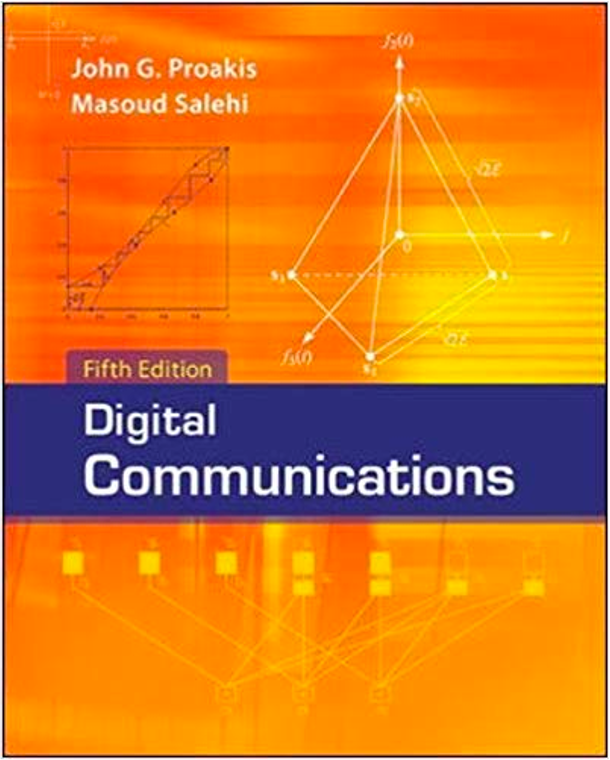
\includegraphics[height=6 cm]{L0_dctextbook.png}
\hspace{1cm}
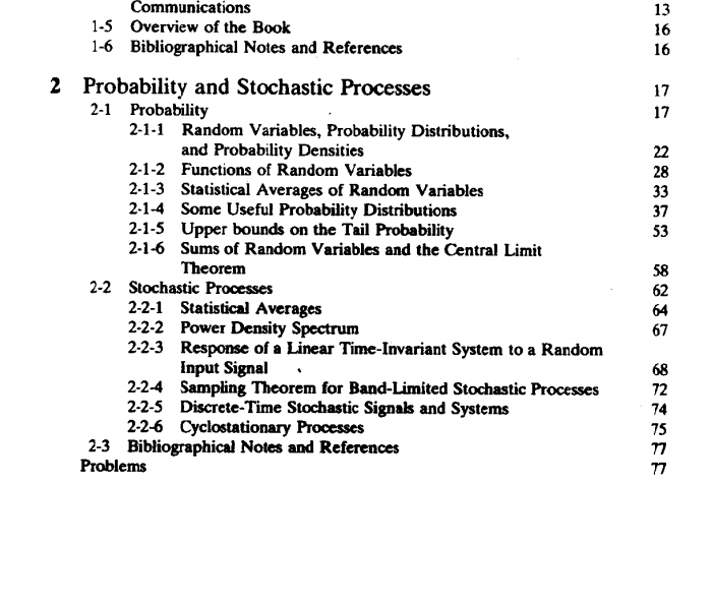
\includegraphics[height=6 cm]{L0_dccontents.png}
\end{frame}

%%%%%%%%%%%%%%%%%%%%%%%%%%%%%%%%%%%%%%%%%%%%%%%%%%%%%%
\begin{frame}{Textbook: Computer Networking}

%\plitemsep 0.1in
\centering
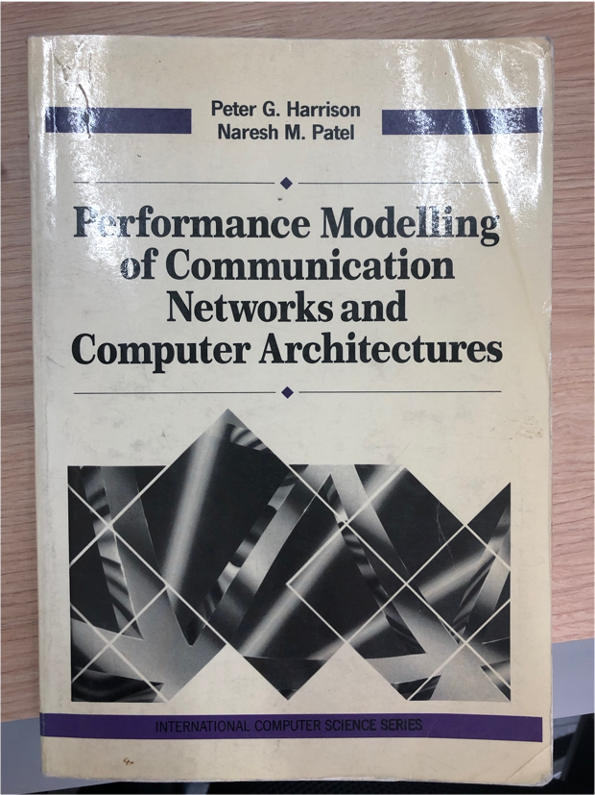
\includegraphics[height=6 cm]{L0_nettextbook.png}
\hspace{1cm}
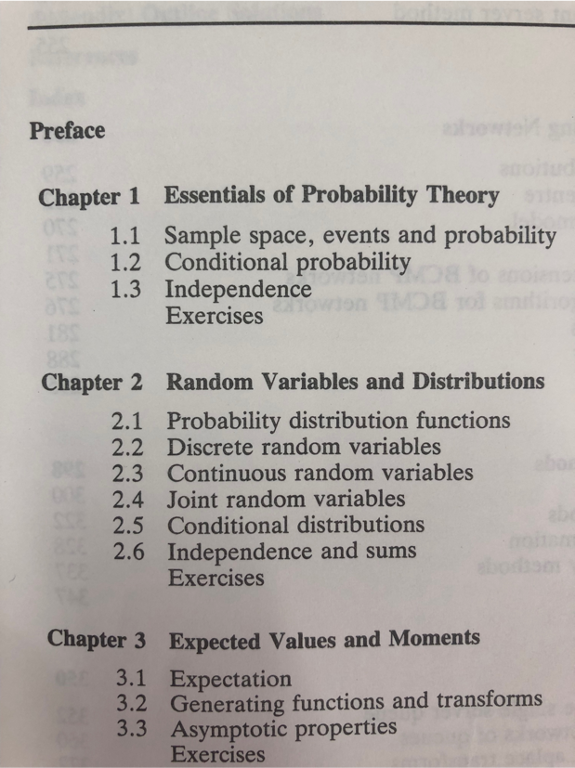
\includegraphics[height=6 cm]{L0_netcontents.png}
\end{frame}

%%%%%%%%%%%%%%%%%%%%%%%%%%%%%%%%%%%%%%%%%%%%%%%%%%%%%%
\begin{frame}{Textbook: Algorithm and Computing}

%\plitemsep 0.1in
\centering
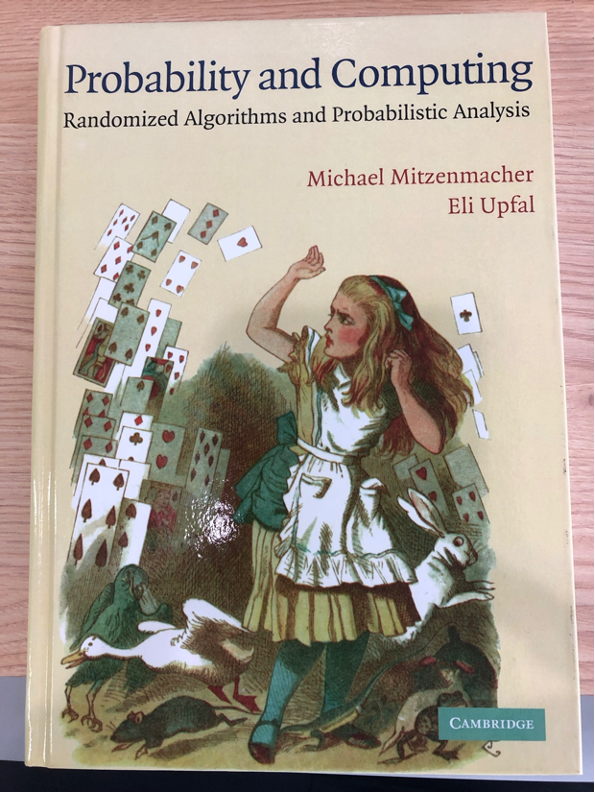
\includegraphics[height=6 cm]{L0_algotextbook.png}
\hspace{1cm}
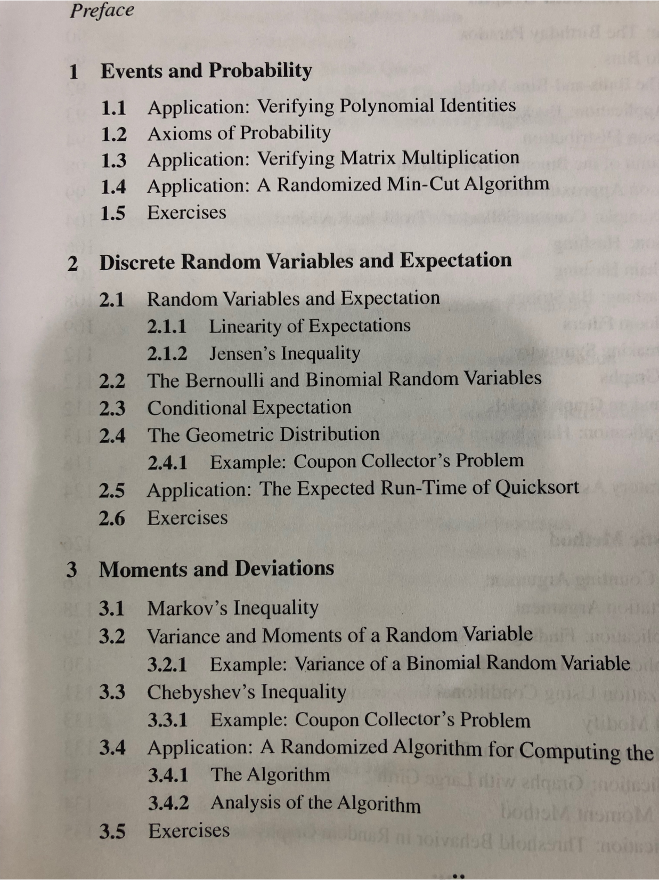
\includegraphics[height=6 cm]{L0_algocontents.png}
\end{frame}

%%%%%%%%%%%%%%%%%%%%%%%%%%%%%%%%%%%%%%%%%%%%%%%%%%%%%%
\begin{frame}{Textbook: Machine Learning}

%\plitemsep 0.1in
\centering
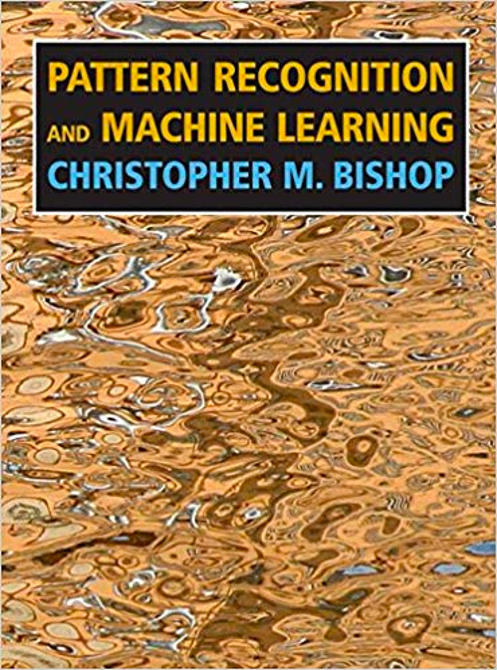
\includegraphics[height=5 cm]{L0_mltextbook.png}
\hspace{0.2cm}
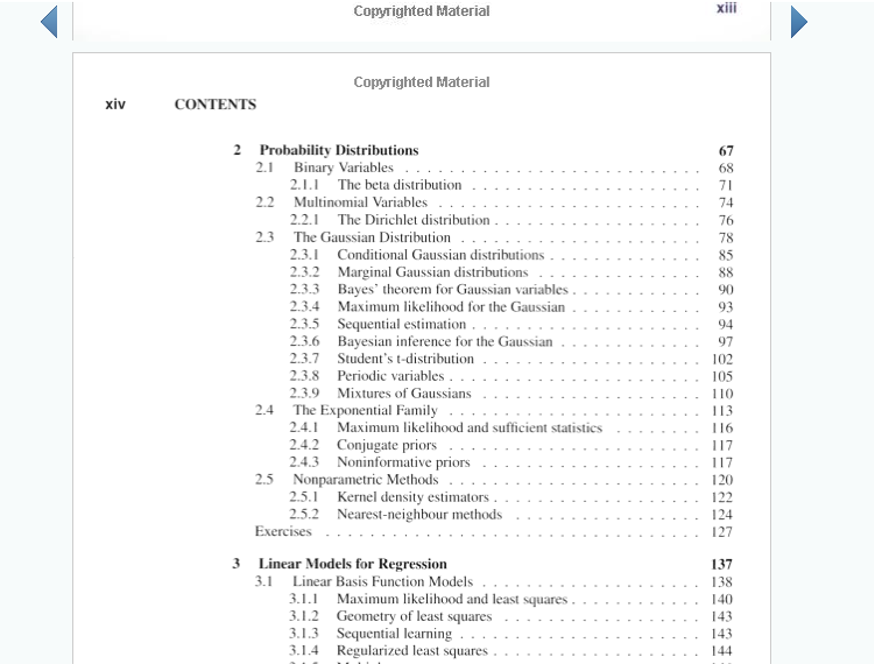
\includegraphics[height=6 cm]{L0_mlcontents.png}

\bigskip

These days, every area in CS and EE is directly or indirectly related to machine learning!
\end{frame}

%%%%%%%%%%%%%%%%%%%%%%%%%%%%%%%%%%%%%%%%%%%%%%%%%%%%%%
\begin{frame}{How to take this course? A designer's perspective}

\bci 

\item<1-> Designer's perspective?

\item<2-> In the year of 2021, suppose that unfortunately there is no theory of mathematically studying
the \empr{uncertainty} of some phenomena, events, etc.  

\item<3-> You have to design such a theory called "probability". How are you going to do it? Where are you going to start? 


\item<3-> You just have other basic mathematical theories such as set theory.

\item<4-> You need to get used to the \redf{English terms} on probability (e.g., sample space = 표본공간, probability density function = 확률밀도함수).

\item<5-> We will take this exciting journey from the next lecture!
\eci

\end{frame}

% %%%%%%%%%%%%%%%%%%%%%%%%%%%%%%%%%%%%%%%%%%%%%%%%%%%%%%
% \begin{frame}{}
% \vspace{2cm}
% \LARGE 나한테 책을 써달라는 부탁을 하는 그림 하나 넣어보자!
% \end{frame}

% %%%%%%%%%%%%%%%%%%%%%%%%%%%%%%%%%%%%%%%%%%%%%%%%%%%%%%
\begin{frame}{}

\mytwocols{0.0}
{
\vspace{2cm}
\centering
\LARGE Questions?
}
{
\centering
\mypic{0.9}{happyjourney.jpg}
}
\end{frame}


\end{document}
